% !TEX root = morphkasten.tex

\section{Antrieb}


%##############
\subsection{DC-Motor}

\begin{figure}[h!]%Position festigen
\centering
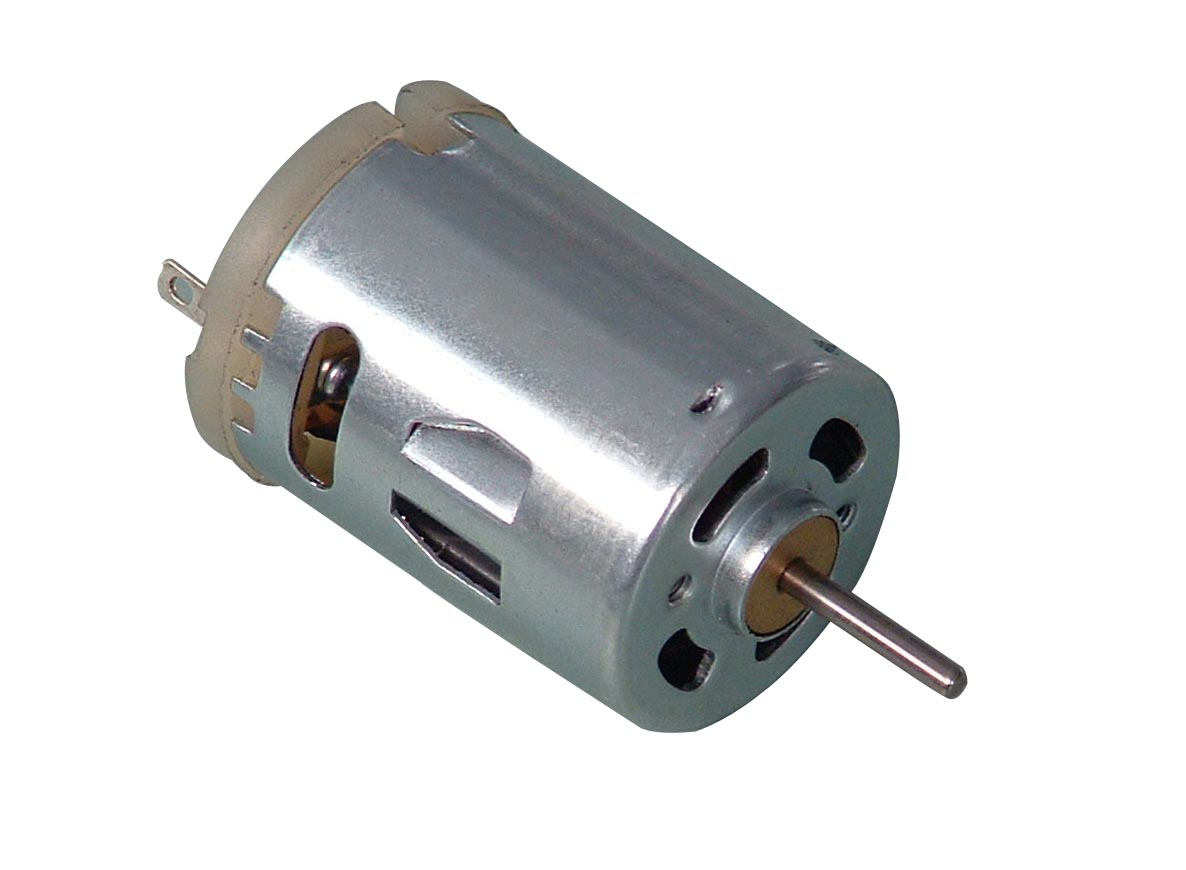
\includegraphics[width=0.5\textwidth]{fig/dcmotor.jpg}
\caption{DC-Motor (Quelle: http://www.mind.ilstu.edu/)}
\label{fig:Java}
\end{figure}

\begin{table}[h]
\begin{tabular}{p{0.5\textwidth} | p{0.5\textwidth}}


 \textbf{Vorteile} & \textbf{Nachteile} \\ \hline
	 
\begin{itemize}
\item Niedriger Anschaffungspreis
\item Simpel in der Handhabung
\item Gut geeignet für permantente Drehung
\end{itemize}

 
 &
 
\begin{itemize}
\item Extra Regelung notwendig
\item Nur bedingt präzise
\item Hohe Wärmeentwicklung
\end{itemize}

\end{tabular}
\end{table}

\begin{table}[h]
\begin{tabular}{p{0.5\textwidth}p{0.5\textwidth}}


 \textbf{Risiken} & \\ \hline
	 
\begin{itemize}
\item Könnte für exaktes Arbeiten (z.B sofortiges Bremsen) zu ungenau sein.
\end{itemize}

 
\end{tabular}
\end{table}

\pagebreak


%##############
\subsection{Schrittmotor}

\begin{figure}[h!]%Position festigen
\centering
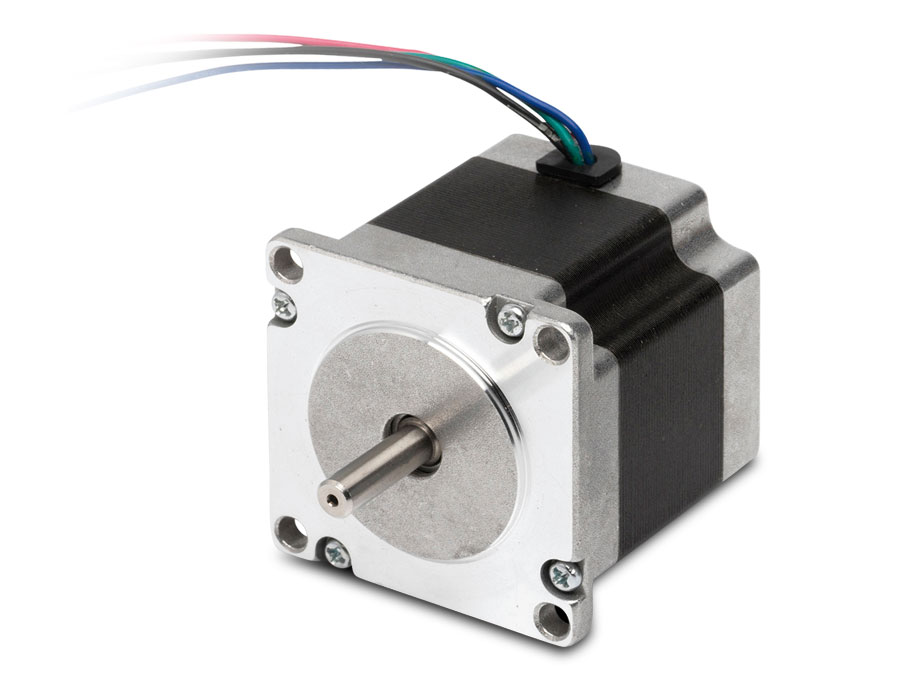
\includegraphics[width=0.5\textwidth]{fig/schrittmotor.JPG}
\caption{Schrittmotor (Quelle: http://www.pollin.de/shop/index.html)}
\label{fig:Java}
\end{figure}

\begin{table}[h]
\begin{tabular}{p{0.5\textwidth} | p{0.5\textwidth}}


 \textbf{Vorteile} & \textbf{Nachteile} \\ \hline
	 
\begin{itemize}
\item Niedriger Anschaffungspreis
\item Genaue Positionsrückmeldung ohne Sensoren
\item Exakte Drehung/Kontrolle
\end{itemize}

 
 &
 
\begin{itemize}
\item Hohe Wärmeentwicklung
\item Hohe Betriebsspannung
\end{itemize}

\end{tabular}
\end{table}

\begin{table}[h]
\begin{tabular}{p{0.5\textwidth}p{0.5\textwidth}}


 \textbf{Risiken} & \\ \hline
	 
\begin{itemize}
\item Es könnten Schrittverluste auftreten
\end{itemize}

 
\end{tabular}
\end{table}

\pagebreak

%##############
\subsection{BLDC-Motor}

\begin{figure}[h!]%Position festigen
\centering
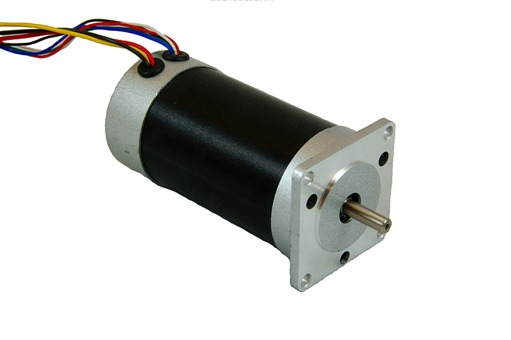
\includegraphics[width=0.5\textwidth]{fig/blcd.jpg}
\caption{BLDC-Motor (Quelle: http://www.ti.com/tool/hvbldcmtr)}
\label{fig:Java}
\end{figure}

\begin{table}[h]
\begin{tabular}{p{0.5\textwidth} | p{0.5\textwidth}}


 \textbf{Vorteile} & \textbf{Nachteile} \\ \hline
	 
\begin{itemize}
\item Niedriger Anschaffungspreis
\item Lange Lebensdauer
\item Hohe Drehzahlen möglich
\item Hoher Wirkungsgrad
\end{itemize}

 
 &
 
\begin{itemize}
\item Extra Regelung notwendig
\end{itemize}

\end{tabular}
\end{table}

\begin{table}[h]
\begin{tabular}{p{0.5\textwidth}p{0.5\textwidth}}


 \textbf{Risiken} & \\ \hline
	 
\begin{itemize}
\item Könnte für exaktes Arbeiten (z.B sofortiges Bremsen) zu ungenau sein.
\end{itemize}

 
\end{tabular}
\end{table}

\pagebreak